\begin{figure}
	\centering
	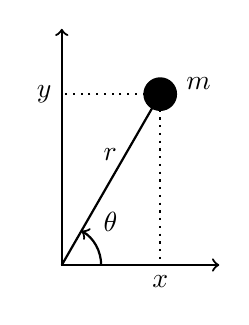
\begin{tikzpicture}[thick]
		\draw [<->,thick] (0,3) |- (2,0);
		\draw [thick] (0,0) -- (1.25, 2.17);
		
		\draw [dotted,thick] (1.25, 2.17) -- (0, 2.17);
		\draw [dotted,thick] (1.25, 2.17) -- (1.25,0);
		
		\draw [fill = black] (1.25,2.17) circle [radius=0.2];
		\draw[->] (0.5,0) arc (0:60:0.5) ;
		
		\node [right] at (1.45,2.3) {$m$};
		\node [right] at (0.4,1.4) {$r$};
		\node [right] at (0.4,0.55) {$\theta$};
		\node [left] at (0, 2.17) {$y$};
		\node [below] at (1.25,0) {$x$};
	\end{tikzpicture}
	\label{fig:examplelagrangian}
	\caption{A free point of mass $m$ in the plane with gravity.}
\end{figure}